\documentclass[a4paper, brazil]{article}
\usepackage[utf8]{inputenc}

\usepackage[cm]{fullpage}
\usepackage{pacotesLaTeX}

\author{Thales Freitas Macêdo \\ DRE: 115 162 177}
\title{LISTA 4}

\begin{document}

\maketitle

\section{Exercício 1}

\begin{figure}[ht]
\centering
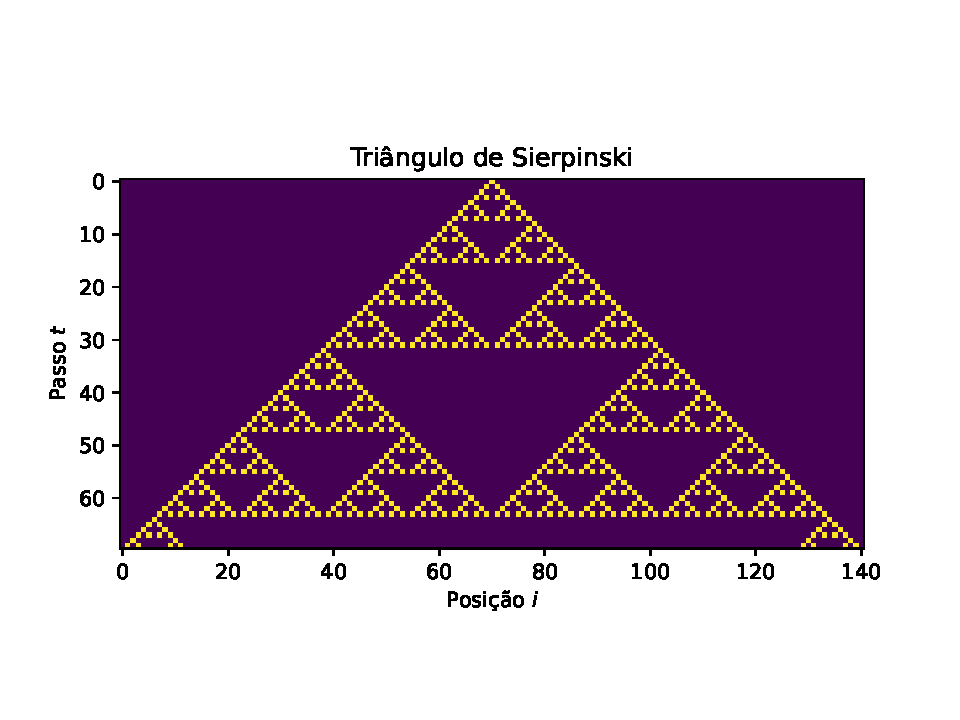
\includegraphics[width=\textwidth]{fig_1.pdf}
\caption{Gráfico do triângulo de Sierpinski gerado pela regra 90, para um vetor inicial de tamanho \( N = 141 \), e um número de passos \( t = 70 \).}\label{fig1}
\end{figure}


\newpage
\section{Exercício 2}

\begin{figure}[ht]
\centering
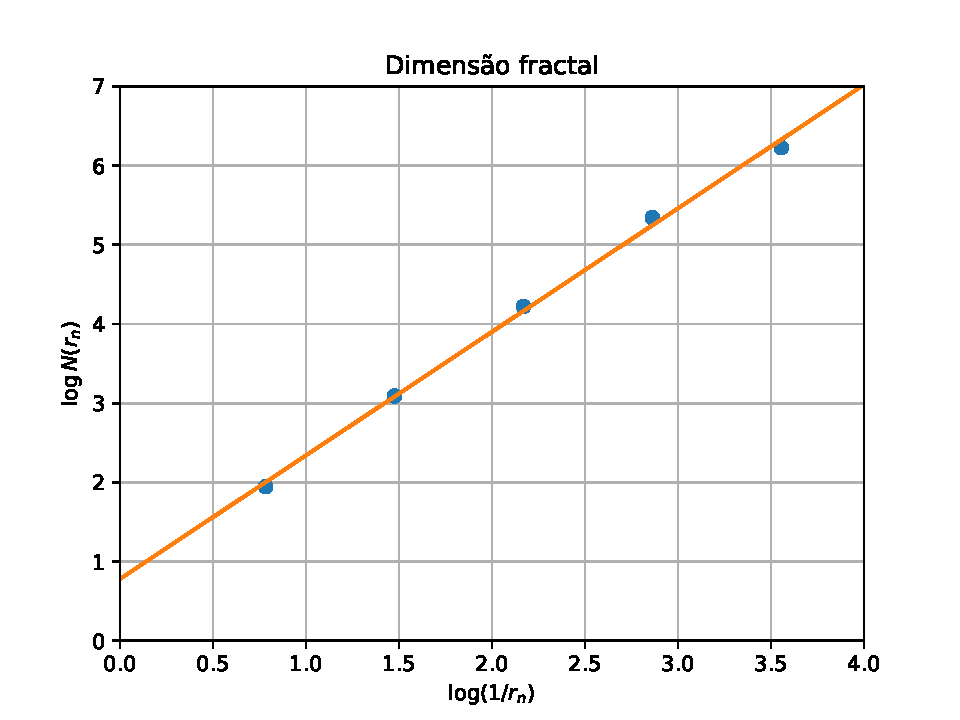
\includegraphics[width=\textwidth]{fig_2.pdf}
\caption{Ajuste linear do gráfico \( \log N(r_n) \times \log(1 / r_n) \), onde \( r_n \) é o tamanho da caixa dividido por 70, e \( N(r_n) \) indica o número de caixas preenchidas para um determinado \( r_n \).
O ajuste linear do gráfico indica um valor de \( d_f = \num{1.56(4)} \), englobando o valor de referência de \( \log(3) / \log(2) \approx \num{1.5850} \).}\label{fig2}
\end{figure}


\newpage
\section{Exercício 3}

\subsection{3.a)}

\begin{figure}[ht]
\centering
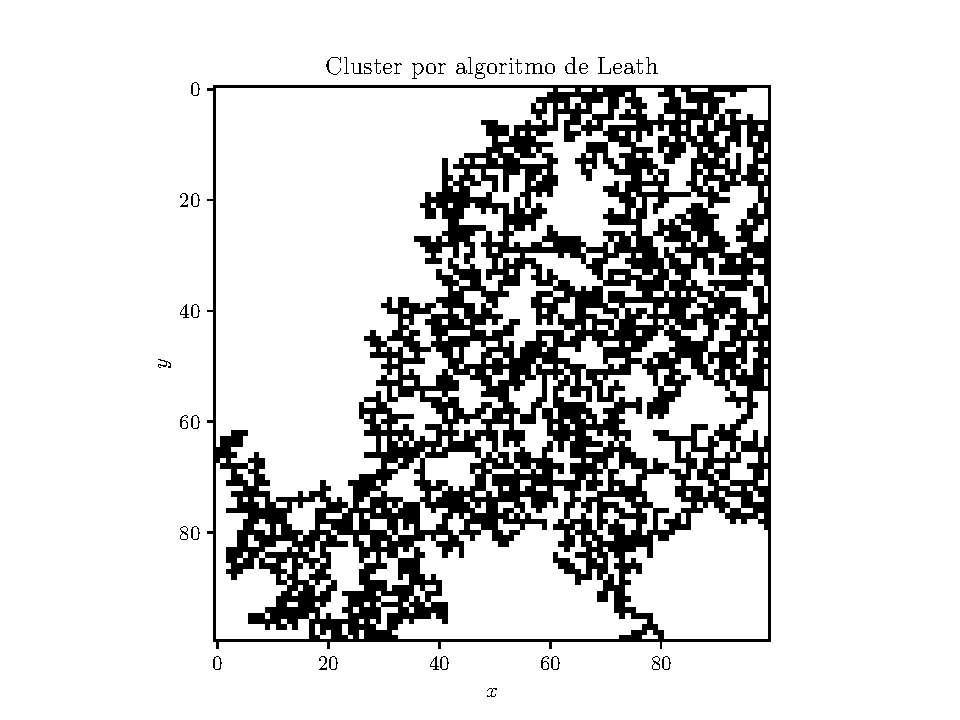
\includegraphics[width=\textwidth]{fig_3a.pdf}
\caption{Gráfico de um cluster de percolação gerado pelo algoritmo de Leath, para uma rede \( L \times L = 100 \times 100 \).}\label{fig3a}
\end{figure}


\newpage
\subsection{3.b)}

\begin{figure}[ht]
    \centering
    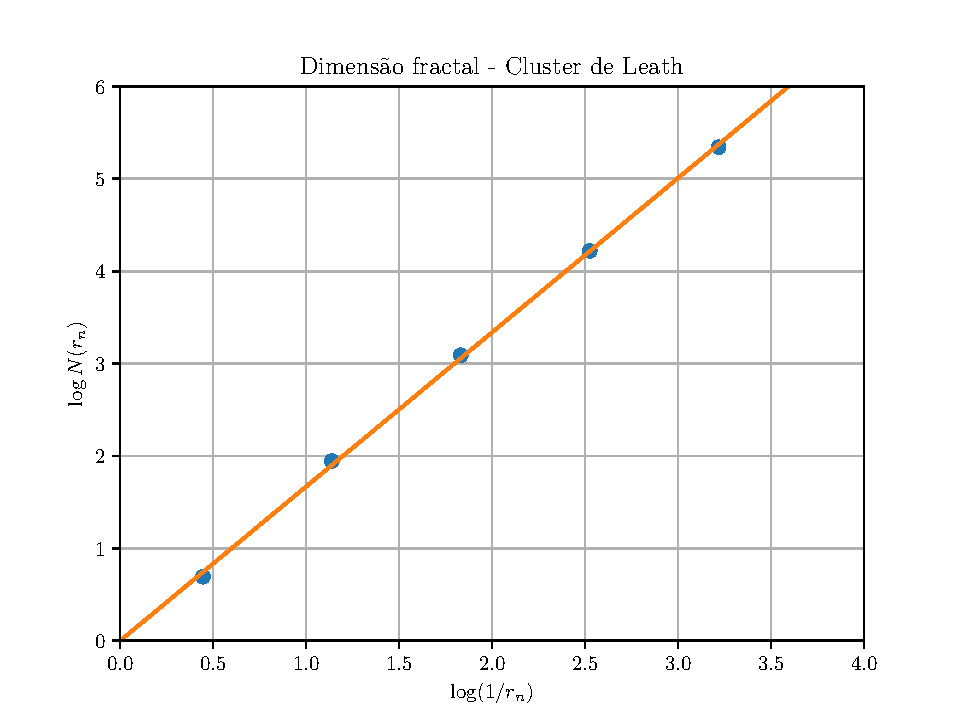
\includegraphics[width=\textwidth]{fig_3b.pdf}
    \caption{Ajuste linear do gráfico \( \log N(r_n) \times \log(1 / r_n) \), onde \( r_n \) é o tamanho da caixa dividido por \( L = 100 \), e \( N(r_n) \) indica o número de caixas preenchidas para um determinado \( r_n \).
    O ajuste linear do gráfico indica um valor de \( d_f = \num{1.67(2)} \).}\label{fig3b}
    \end{figure}

\newpage
\subsection{3.c)}

\begin{figure}[ht]
    \centering
    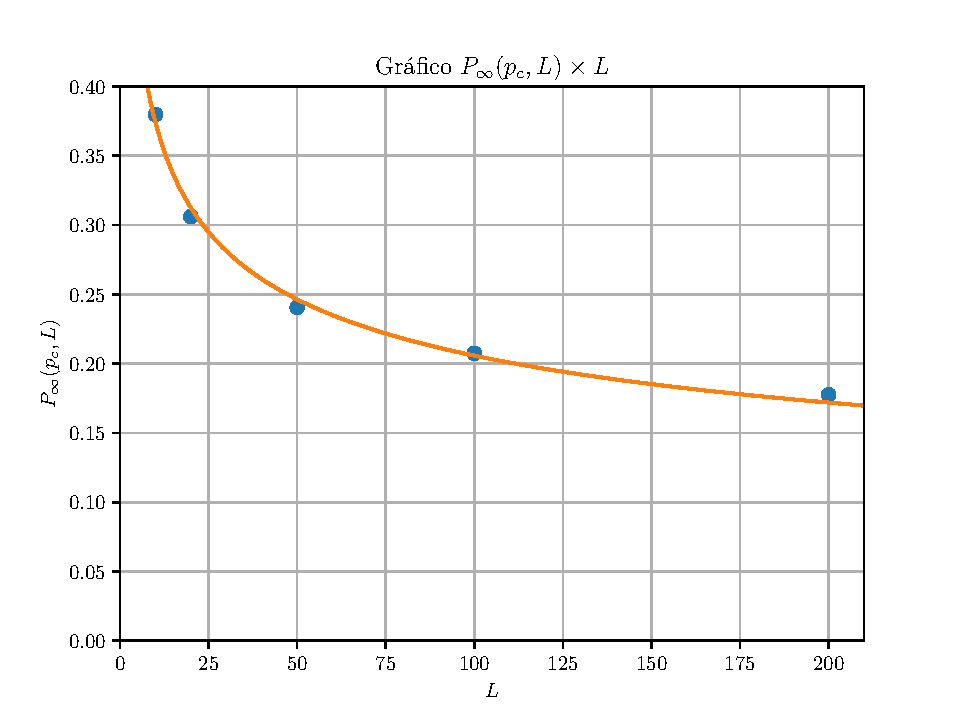
\includegraphics[width=\textwidth]{fig_3c.pdf}
    \caption{Ajuste à equação \( y = A x^k \) do gráfico \( P_\infty (p_c, L) \times L \) obtido por uma estatística de 10000 clusters..
    O ajuste fornece os valores \( A = \num{0.68(3)} \) e \( k = \num{-0.26(1)} \), de onde estimo que \( \beta / \nu = \num{0.26} \).}\label{fig3c}
    \end{figure}

\newpage
\subsection{3.d)}

\begin{figure}[ht]
    \centering
    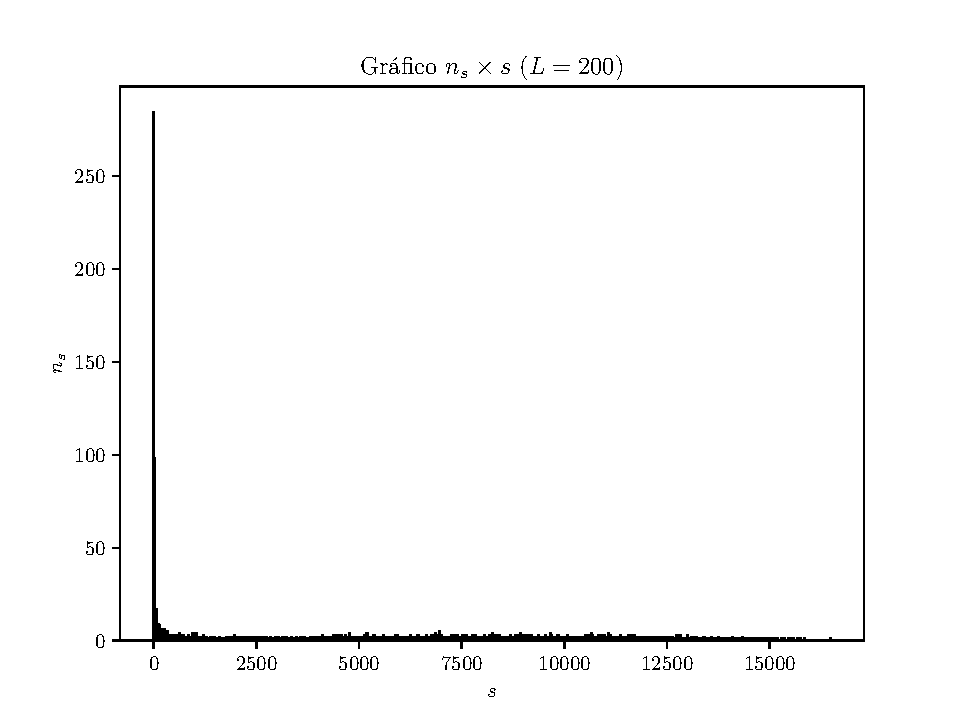
\includegraphics[width=\textwidth]{fig_3d.pdf}
    \caption{Gráfico da distribuição \( n_s \) de clusters de tamanho \( s \), com o descarte dos clusters de percolação, e uma estatística de 10000 clusters.
    A distribuição ficou concentrada em \( s = 1\), caindo drasticamente para os valores segiuntes de \( s \).}\label{fig3d}
    \end{figure}

\end{document}
